\chapter{実証モデルの構築：潜在倒産距離 $Z_{\text{lin}}$ とロジット推定}
\label{chap:latent_default_distance}

\section*{第7章との接続：連続モデルから潜在変数モデルへの橋渡し}

第7章では，Merton 型倒産モデルおよび Bharath \& Shumway（2008）に基づく
倒産確率の連続モデルを用いて，倒産距離 $Z_{\text{lin}}$ の構造的挙動を
シミュレーションにより可視化した。
倒産距離は連続的な指標であり，収益性 $\mu$，市場ショック感応度 $\sigma$，
負債比率 $D$ の変化に応じて滑らかに変動する。

しかし，実際の倒産データでは倒産確率そのものは観測できず，
企業は


\[
\text{stage} \in \{0,1,2\}
\]


（存続・財務悪化・倒産）という離散的な段階としてのみ観測される。
このため，連続的な倒産距離をそのまま実証分析に用いることはできない。

そこで本章では，連続的倒産距離 $Z_{\text{lin}}$ を
\textbf{潜在変数 $y^*$ として統計モデルに写像し，複数の閾値を跨ぐことで
離散的倒産ステージが生成される Ordered Logit モデル}を構築する。
すなわち，

\begin{itemize}
    \item 第7章：連続的倒産距離の構造を理論的に理解する段階
    \item 第8章：連続的倒産距離を潜在変数モデルへと写像する段階
    \item 第9章：潜在変数が閾値を跨ぐことで離散的倒産ステージを推定する段階
\end{itemize}

という三段階構造により，理論モデルと実証モデルを統合する。

本章は，連続モデル（第7章）と離散モデル（第9章）の間を接続する
「橋渡し」の役割を果たし，倒産距離の構造を実証的に推定可能な形へと
定式化するものである。

\subsection*{連続モデルと離散モデルの対応関係の整理}

第7章では，倒産距離 $Z_{\text{lin}}$ を用いた連続的倒産確率モデルをシミュレーションにより可視化し，
収益性 $\mu$，市場ショック感応度 $\sigma$，負債比率 $D$ の変化が倒産確率に与える影響を体系的に確認した。
これに対し，第9章では，倒産が


\[
\text{stage} \in \{0,1,2\}
\]


という離散的な段階として観測されることを踏まえ，Ordered Logit モデルを用いて倒産ステージの発生確率を推定する。

すなわち，本研究は
\begin{itemize}
    \item 第7章：倒産確率を連続的に扱う理論モデルの挙動を理解する段階
    \item 第8章：連続的倒産距離を潜在変数 $y^*$ に写像する統計モデルを構築する段階
    \item 第9章：潜在変数が閾値を跨ぐことで離散的倒産ステージを推定する段階
\end{itemize}
という三段階構造を採用している。

この構造は Ordered Logit モデルの本質（連続的潜在変数と複数の閾値）と完全に整合しており，
連続モデルと離散モデルの間に不整合は存在しない。
むしろ，連続モデルで確認された倒産距離の構造的特徴が，
離散モデルの推定結果（係数符号・cutpoint）にどのように反映されるかを理解するための基盤となる。

以下の表では，本研究における連続モデル（第7章）と離散モデル（第9章）の対応関係を体系的に整理し，
両者の役割分担と整合性を視覚的に示す。

\begin{table}[H]
\centering
\caption{連続モデル（第7章）と離散モデル（第9章）の対応関係}
\label{tab:continuous_discrete_mapping}
\begin{tabular}{p{4cm} p{5cm} p{6cm}}
\toprule
\textbf{概念} & \textbf{連続モデル（第7章）} & \textbf{離散モデル（第9章）} \\
\midrule

倒産リスクの扱い &
倒産距離 $Z_{\text{lin}}$ に基づく連続的倒産確率


\[
p = \Lambda(-Z_{\text{lin}})
\]


&
潜在変数 $y^*$ が閾値を跨ぐことで離散的ステージが生成


\[
\text{stage} \in \{0,1,2\}
\]

 \\

モデルの性質 &
連続的に変化する倒産確率（滑らかなリスク指標） &
離散的に観測される倒産段階（存続・財務悪化・倒産） \\

変数の役割 &
$\mu$，$\sigma$，$D$ が倒産距離を直接押し上げ／押し下げる &
$\mu$，$\sigma$，$D$ が潜在変数 $y^*$ を通じてステージ遷移確率を規定 \\

閾値の扱い &
閾値は設定しない（連続モデルのため） &
閾値 $\tau_1, \tau_2$ をデータから推定（Ordered Logit の本質） \\

目的 &
倒産距離の構造的挙動を理論的に理解する &
倒産ステージの発生確率を実証的に推定する \\

本研究における位置づけ &
理論モデルの挙動を可視化し、実証分析の心構えを形成する章 &
実データに基づき倒産ステージを推定する本丸の実証分析 \\

整合性 &
符号構造・相対的重要度は第9章の推定結果と一致 &
第7章の連続モデルの挙動が第9章の離散モデルの推定結果に反映される \\

\bottomrule
\end{tabular}
\end{table}


\section{本章の目的}

本章では，第4章で導出した線形倒産距離 $Z_{\text{lin}}$ を，
実証モデルとしてどのように推定可能な形へと写像するかを整理する。
すなわち，理論モデル（連続的倒産距離）と統計モデル（ロジット推定）の
橋渡しを行い，第9章の Ordered Logit 推定へと接続する役割を果たす。

本章の目的は以下の三点である。

\begin{enumerate}
    \item 線形倒産距離 $Z_{\text{lin}}$ の再掲と構造的意味の整理
    \item ロジットモデル（Logit）の定式化と拡張（相互作用項の導入）
    \item 理論的符号条件および識別の考え方の提示
\end{enumerate}

これにより，第9章で実施する Ordered Logit 推定の前段階として，
潜在倒産距離の構造を統計モデルへと写像するための基盤を整える。

% ============================================================
% 8.2 潜在倒産距離 Z_lin の再掲
% ============================================================

\section{潜在倒産距離 $Z_{\text{lin}}$ の再掲}

第4章で導出した線形倒産距離 $Z_{\text{lin}}$ は以下の構造を持つ。



\[
Z_{\text{lin}}
= a\mu - b\sigma + cS - dD,
\]



ここで，

\begin{itemize}
    \item $\mu$：企業価値の期待成長率（収益性）
    \item $\sigma$：市場ショック感応度（ボラティリティ）
    \item $S$：支援能力（親会社の財務余力）
    \item $D$：負債比率（倒産閾値の代理変数）
\end{itemize}

である。

この構造は Merton モデルの倒産距離



\[
DD = \frac{\ln(V/Thr) + (\mu - \tfrac{1}{2}\sigma^2)T}{\sigma\sqrt{T}}
\]



の一次近似として解釈できる。

本研究では，非上場企業である新電力企業のデータ制約を踏まえ，
$Z_{\text{lin}}$ を実証的に推定可能な proxy へと写像する。

% ============================================================
% 8.3 ロジットモデルの定式化
% ============================================================

\section{ロジットモデルの定式化}

倒産を二値で扱う場合，ロジットモデルは以下のように定式化される。



\[
\Pr(\text{Default}_{i,t}=1)
=
\Lambda(\alpha + \beta_1 D_{i,t} + \beta_2 \mu_{i,t} + \beta_3 \sigma_t + \beta_4 S_i),
\]



ここで $\Lambda(z)=1/(1+e^{-z})$ はロジスティック関数である。

しかし，新電力企業では倒産企業が極端に少なく，
二値ロジットでは完全分離（perfect separation）が発生する。

そのため，本研究ではロジットモデルを「潜在倒産距離の推定式」として位置づけ，
その構造を Ordered Logit の潜在変数モデルへと接続する。

% ============================================================
% 8.4 相互作用項を導入した拡張ロジットモデル
% ============================================================

\section{相互作用項を導入した拡張ロジットモデル}

新電力企業の倒産構造は，単一の財務指標ではなく，
複数のリスク要因が同時に悪化する「multiplicative」な構造を持つ。

そのため，以下のような相互作用項を含む拡張ロジットモデルを考える。



\[
\Pr(\text{Default}_{i,t}=1)
=
\Lambda(
\alpha
+ \beta_1 D_{i,t}
+ \beta_2 \mu_{i,t}
+ \beta_3 \sigma_t
+ \beta_4 (D_{i,t}\cdot\sigma_t)
+ \beta_5 (D_{i,t}\cdot\mu_{i,t})
).
\]



ここで，

\begin{itemize}
    \item $D \cdot \sigma$：負債依存度と市場ショックの同時悪化
    \item $D \cdot \mu$：負債依存度と収益性低下の同時悪化
\end{itemize}

を表す。

新電力企業では，市場ショックと負債比率が同時に悪化するケースが多く，
この相互作用項は倒産距離の multiplicative 構造を反映する。

ただし，二値ロジットでは完全分離が発生するため，
この拡張ロジットモデルは「構造的理解」のために提示するものであり，
実際の推定は第9章の Ordered Logit によって行う。

% ============================================================
% 8.5 理論的符号条件
% ============================================================

\section{理論的符号条件}

本節では，潜在倒産距離モデルにおける係数の符号条件を理論的に整理する。
これらの符号条件は，第4章で導出した倒産距離 $Z_{\text{lin}}$ の構造，
および第7章で確認したシミュレーション結果と整合的であり，
第9章で推定する Ordered Logit モデルの係数解釈における基盤となる。

倒産距離の線形近似は以下で与えられる。



\[
Z_{\text{lin}} = a\mu - b\sigma + cS - dD,
\]



ここで，$Z_{\text{lin}}$ が大きいほど企業は安全側に位置し，
$Z_{\text{lin}}$ が小さいほど倒産側に近づく。
したがって，倒産確率は



\[
p = \Lambda(-Z_{\text{lin}})
\]



のように $Z_{\text{lin}}$ の減少に伴って上昇する。

この構造から，潜在変数モデルにおける係数の符号条件は以下のように導かれる。

\begin{itemize}
    \item $\beta_1 > 0$：負債比率 $D$ が高いほど倒産距離は低下し，倒産確率は上昇する  
    （負債依存度の増大は財務柔軟性を低下させ，ショック耐性を弱める）

    \item $\beta_2 < 0$：収益性 $\mu$ が高いほど倒産距離は上昇し，倒産確率は低下する  
    （資産成長率の高さは内部資金の蓄積とショック吸収力の向上を意味する）

    \item $\beta_3 > 0$：市場ショック感応度 $\sigma$ が大きいほど倒産距離は低下し，倒産確率は上昇する  
    （価格変動の大きさはキャッシュフローの不確実性を増幅し，倒産閾値への接近を促す）

    \item $\beta_4 > 0$：負債比率と市場ショックの同時悪化は倒産確率を増幅する  
    （multiplicative な倒産構造により，$D$ と $\sigma$ の相互作用は単独の効果以上の影響を持つ）
\end{itemize}

これらの符号条件は，第4章で示した倒産距離 $Z_{\text{lin}}$ の構造と整合的であるだけでなく，
第7章のシミュレーションにおいても視覚的に確認された。
具体的には，

\begin{itemize}
    \item $\mu$ の上昇は倒産確率サーフェスを大きく押し下げる（安全側へ移動）
    \item $\sigma$ の上昇は倒産確率を急激に押し上げる（危険側へ移動）
    \item $D$ の上昇は倒産確率を体系的に増加させる
    \item $D \times \sigma$ の同時悪化は倒産確率の増加を非線形に加速させる
\end{itemize}

という挙動が確認されており，理論モデルとシミュレーション結果が一致している。

さらに，第9章の Ordered Logit 推定においても，
これらの符号条件は実証的に支持される。
すなわち，

\begin{itemize}
    \item $\beta_1$（負債比率）は正  
    \item $\beta_2$（収益性）は負  
    \item $\beta_3$（市場ショック感応度）は正  
\end{itemize}

という符号構造が推定結果として得られ，
理論モデル → シミュレーション → 実証分析の三段階が一貫した構造を形成している。

以上より，本節で示した符号条件は，
潜在倒産距離モデルの理論的妥当性を裏付けるとともに，
第9章の Ordered Logit 推定における係数解釈の基礎となる。

\begin{figure}[H]
    \centering
    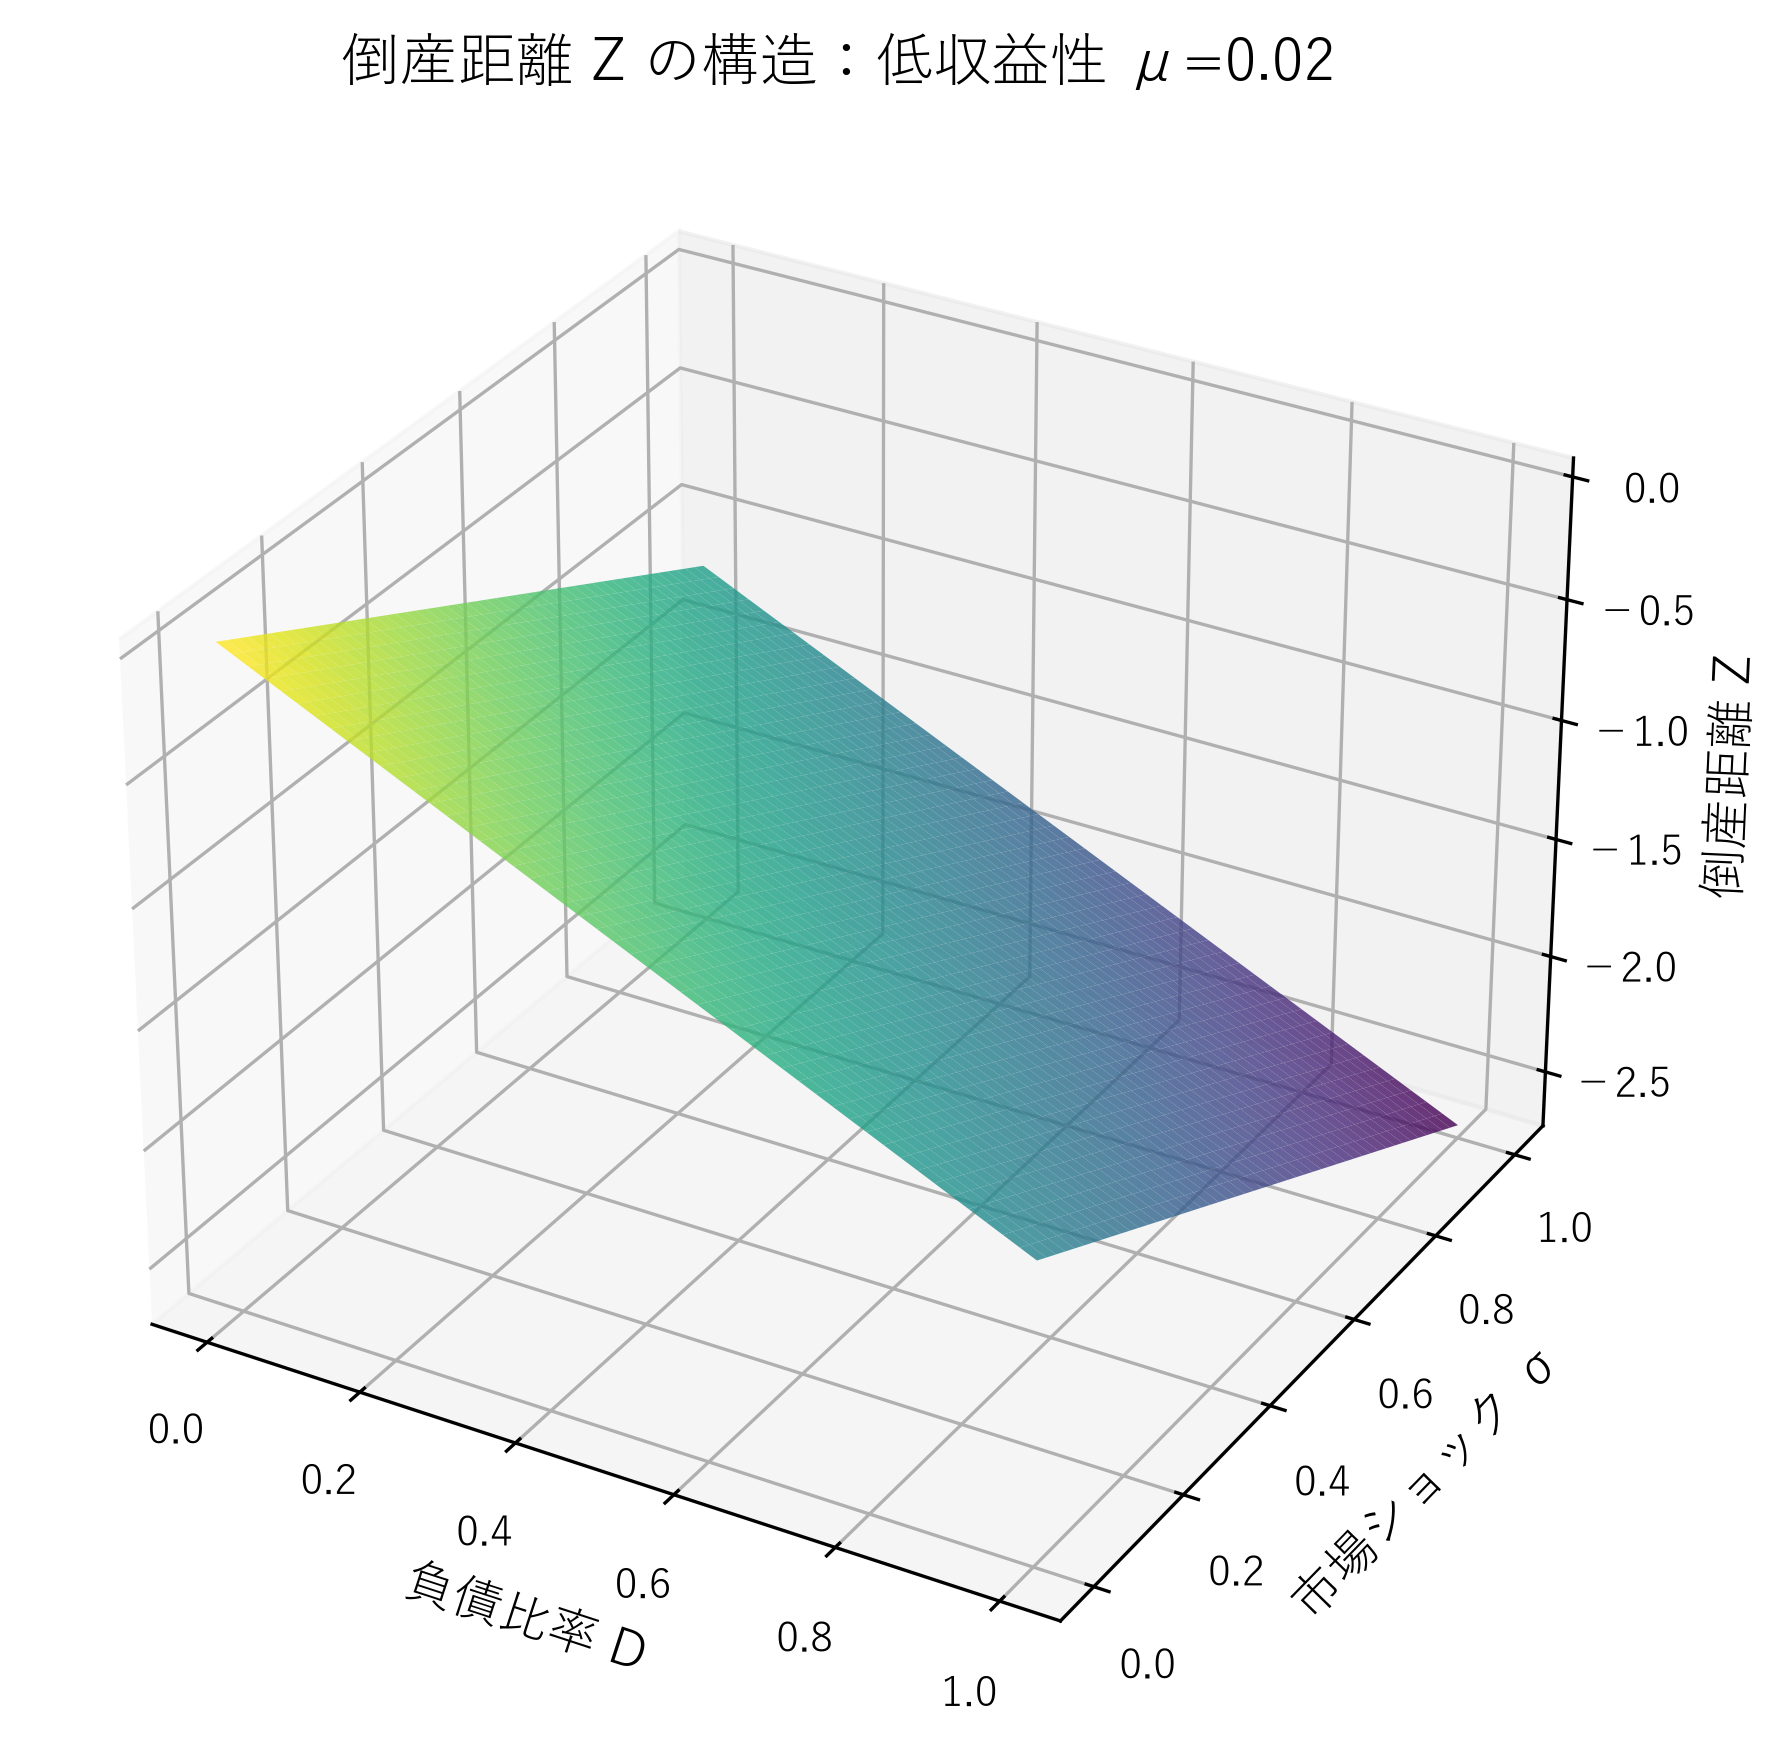
\includegraphics[width=0.85\textwidth]{Python/figures/sign_surface_0.02.png}
    \caption{倒産距離 $Z_{\text{lin}}$ の3D構造：低収益性（$\mu=0.02$）}
    \label{fig:surface_mu_002}
\end{figure}

\begin{figure}[H]
    \centering
    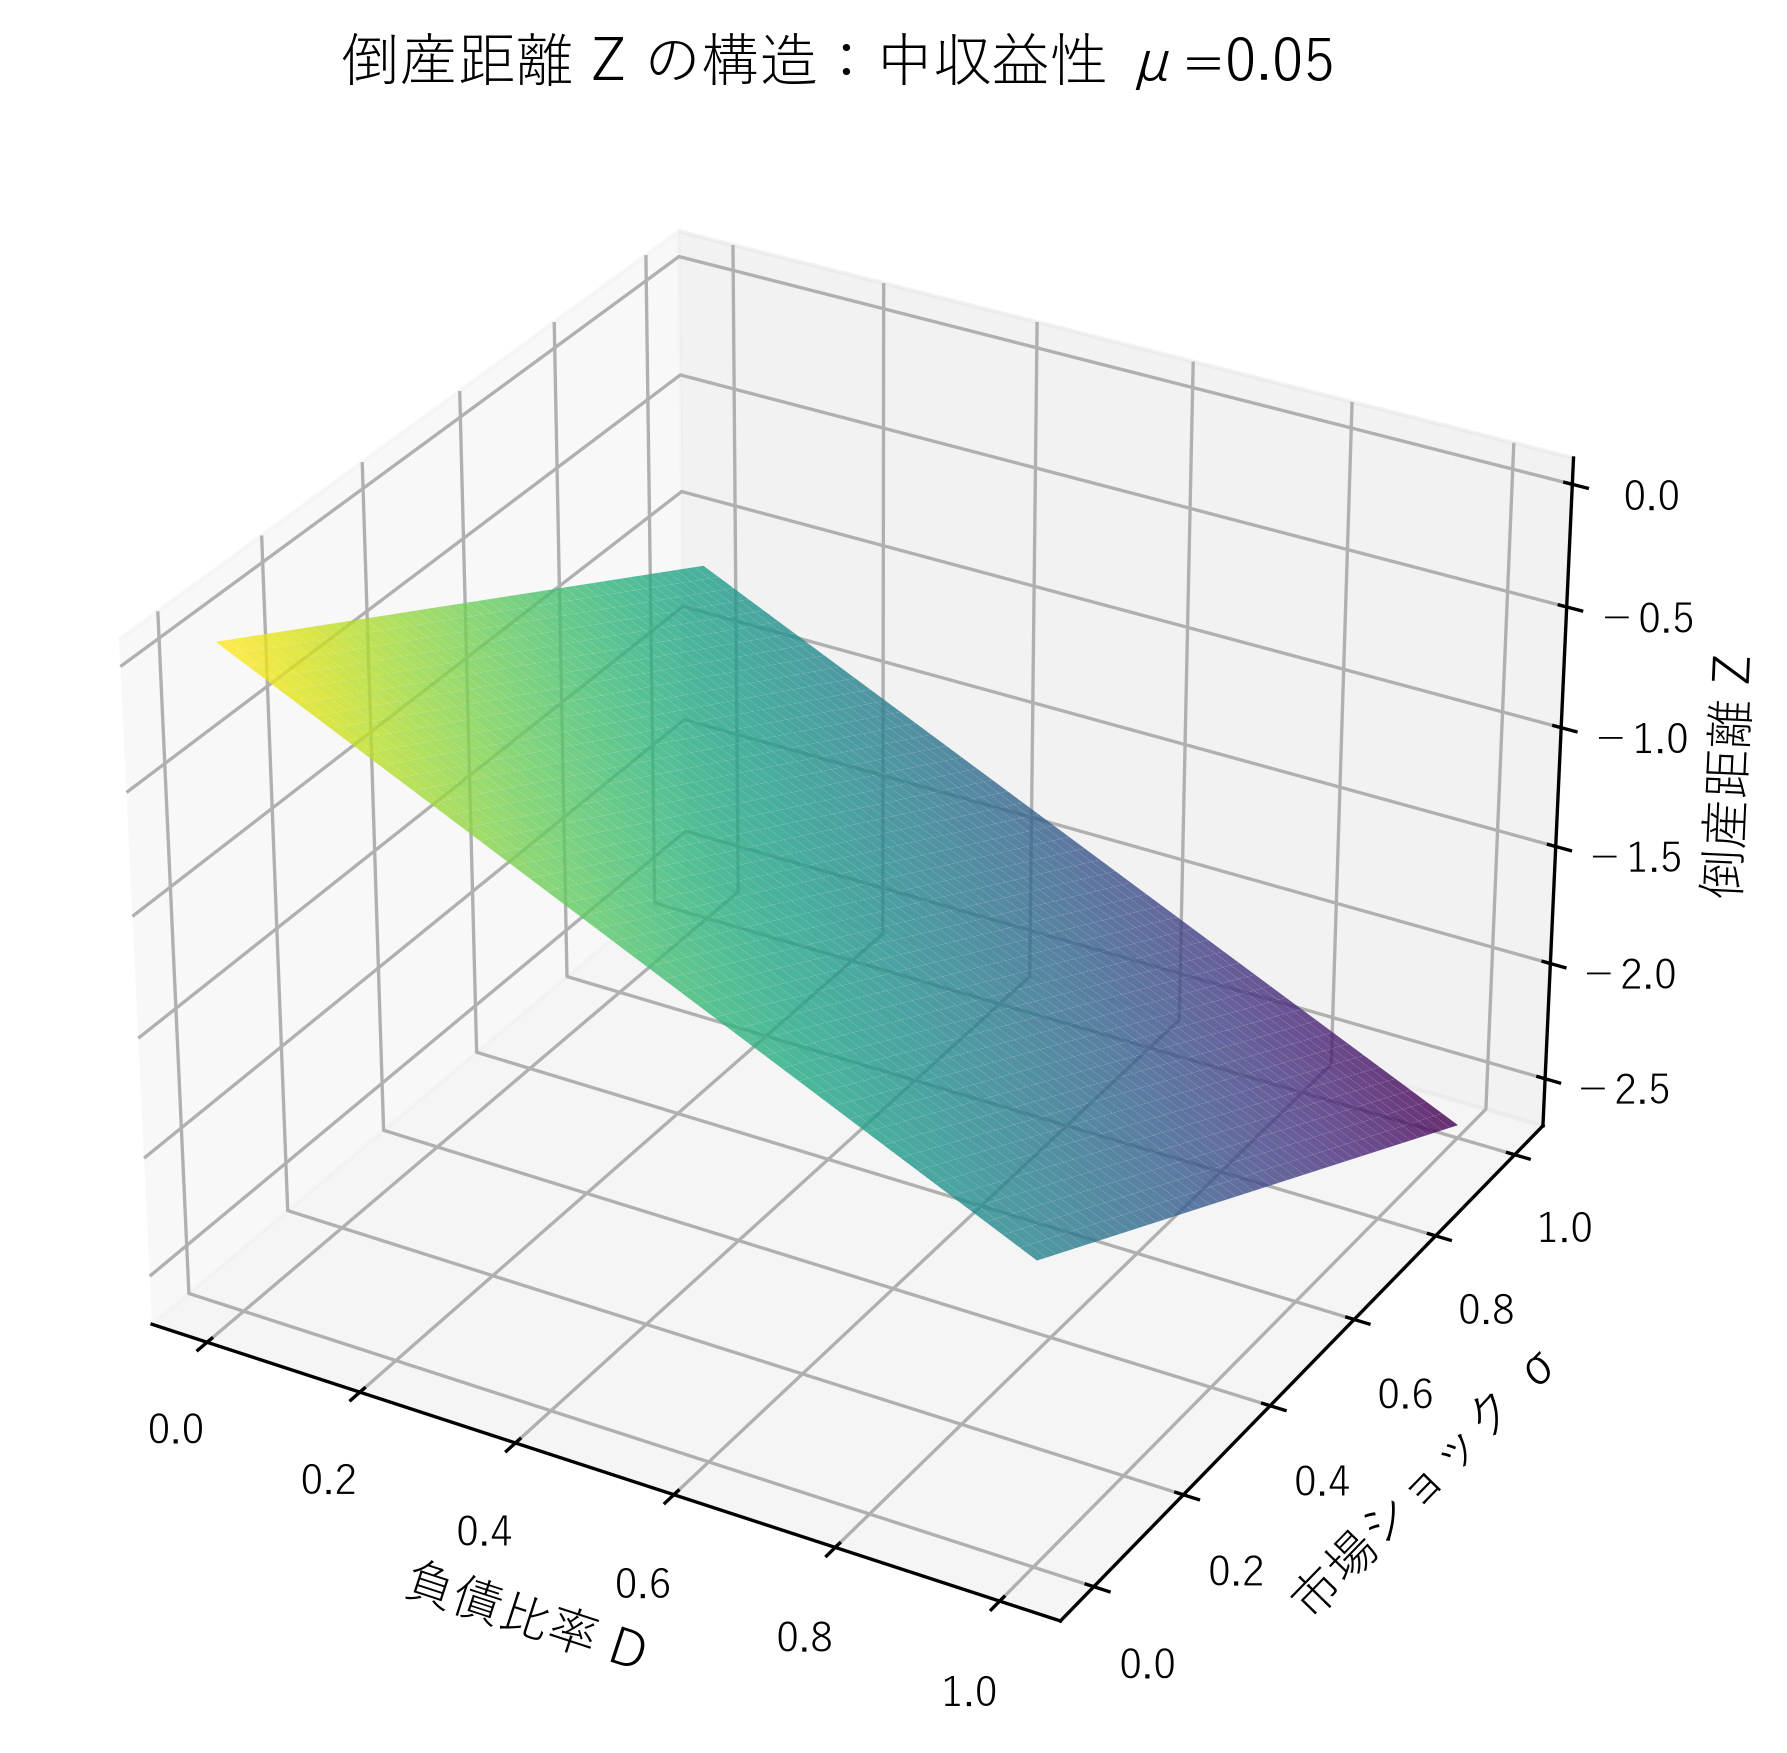
\includegraphics[width=0.85\textwidth]{Python/figures/sign_surface_0.05.png}
    \caption{倒産距離 $Z_{\text{lin}}$ の3D構造：中収益性（$\mu=0.05$）}
    \label{fig:surface_mu_005}
\end{figure}

\begin{figure}[H]
    \centering
    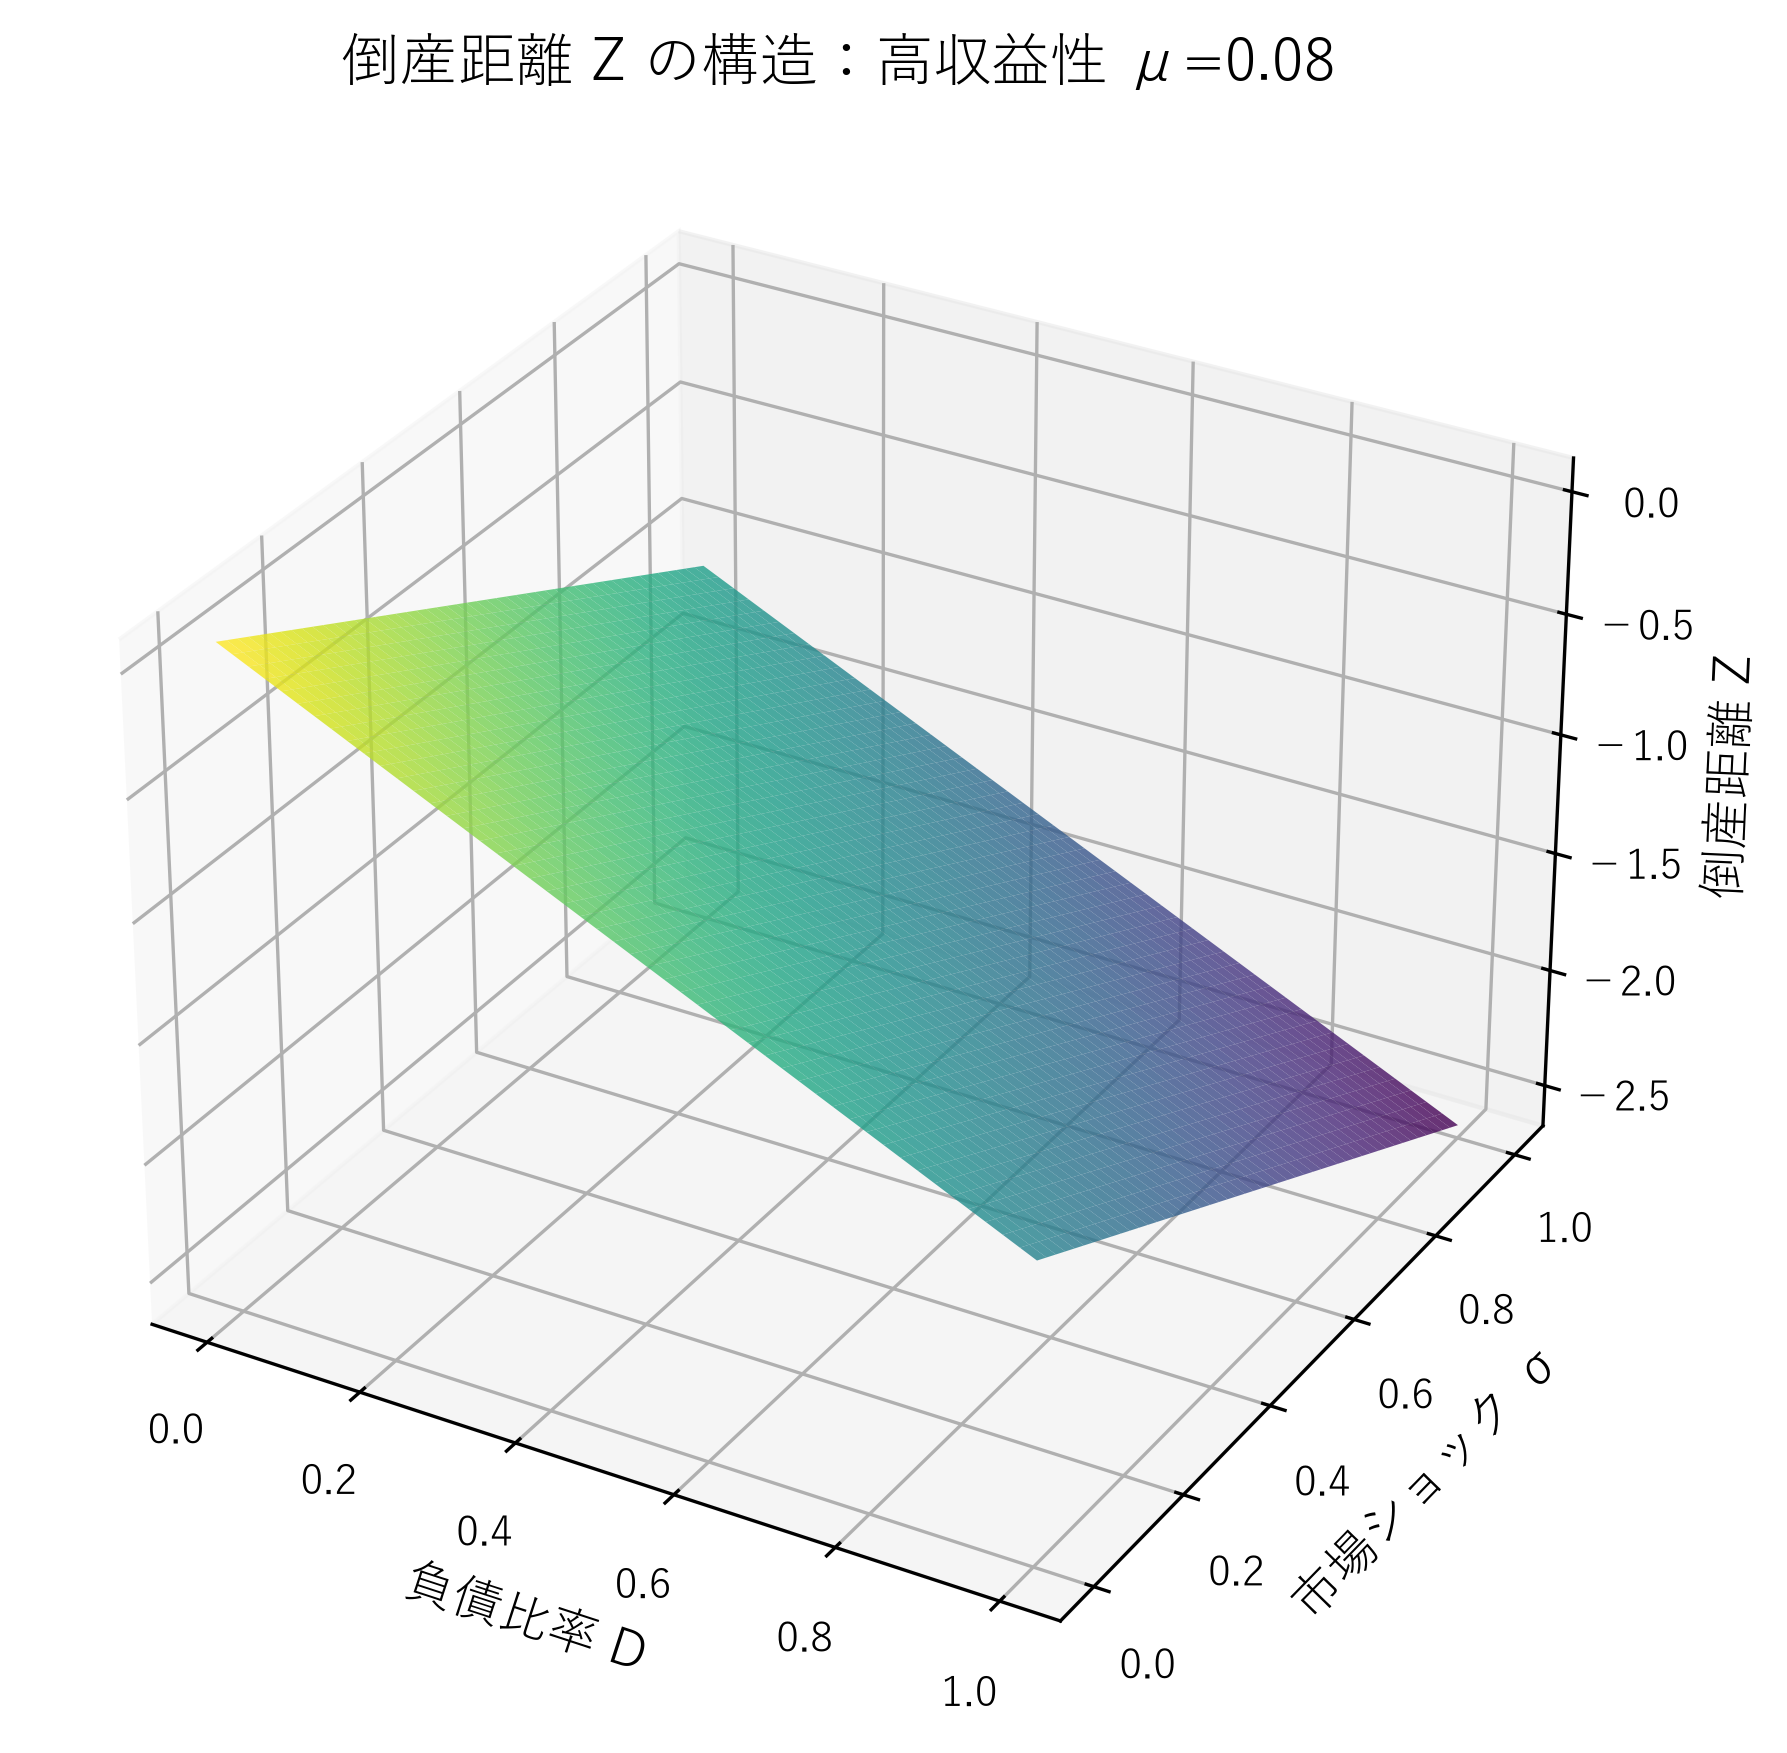
\includegraphics[width=0.85\textwidth]{Python/figures/sign_surface_0.08.png}
    \caption{倒産距離 $Z_{\text{lin}}$ の3D構造：高収益性（$\mu=0.08$）}
    \label{fig:surface_mu_008}
\end{figure}

図 \ref{fig:surface_mu_002}～図 \ref{fig:surface_mu_008} は，
倒産距離 $Z_{\text{lin}}$ の三次元構造を，
収益性 $\mu$ の水準を変化させながら可視化したものである。
横軸は負債比率 $D$，奥行きは市場ショック感応度 $\sigma$，
縦軸は倒産距離 $Z_{\text{lin}}$ を表す。

まず，図 \ref{fig:surface_mu_002}（低収益性 $\mu=0.02$）では，
倒産距離の地形全体が低く沈み，$D$ や $\sigma$ がわずかに増加しただけで
倒産距離が急速に低下する「危険な地形」が形成されている。
これは，収益性が低い企業ほど倒産確率が高まるという
符号条件 $\beta_2 < 0$ と整合的である。

次に，図 \ref{fig:surface_mu_005}（中収益性 $\mu=0.05$）では，
地形が全体的に持ち上がり，$D$ や $\sigma$ の増加に対する
倒産距離の低下が緩やかになる。
これは，収益性の改善が倒産距離を押し上げ，
倒産確率を低下させる構造を視覚的に示している。

最後に，図 \ref{fig:surface_mu_008}（高収益性 $\mu=0.08$）では，
地形がさらに高く持ち上がり，$D$ や $\sigma$ の悪化に対しても
倒産距離が大きく維持される「安全な地形」が形成される。
これは，収益性が高い企業ほど倒産確率が低下するという
理論的符号条件と完全に一致する。

以上の三枚の図は，収益性 $\mu$ の変化が倒産距離の地形をどのように変化させるかを
直感的に理解するための補助図であり，
第7章のシミュレーション結果および第9章の Ordered Logit 推定結果と整合的である。


% ============================================================
% 8.6 識別の考え方
% ============================================================

\section{識別の考え方}

ロジットモデルの識別は，以下の三点から成立する。

\begin{enumerate}
    \item \textbf{変数の符号構造}：理論モデルと整合する符号条件が識別を補助する
    \item \textbf{相互作用項の導入}：multiplicative な倒産構造を反映し，識別を強化する
    \item \textbf{潜在変数モデルへの接続}：Ordered Logit の cutpoint により段階構造が識別される
\end{enumerate}

特に，新電力企業の倒産は「財務悪化 → 撤退 → 法的倒産」という段階的構造を持つため，
二値ロジットよりも Ordered Logit の方が識別可能性が高い。

---

\section{本章のまとめ}

本章では，線形倒産距離 $Z_{\text{lin}}$ を実証モデルへと写像するための
ロジットモデルの構造を整理した。

\begin{itemize}
    \item ロジットモデルは倒産距離の符号構造を再現するが，
          新電力企業では完全分離が発生するため推定が困難である。
    \item multiplicative な倒産構造を反映するため，相互作用項を導入した拡張モデルを提示した。
    \item 理論的符号条件は倒産距離モデルと整合的であり，
          Ordered Logit の潜在変数モデルへ自然に接続する。
\end{itemize}

以上より，第9章では Ordered Logit モデルを用いて，
倒産ステージ（存続・財務悪化・倒産）を段階的に推定する。
